
\documentclass[11pt,a4paper]{report}%especifica o tipo de documento que tenciona escrever: carta, artigo, relatório... neste caso é um relatório
% [11pt,a4paper] Define o tamanho principal das letras do documento. caso não especifique uma delas, é assumido 10pt
% a4paper -- Define o tamanho do papel.

\usepackage[portuges]{babel}%Babel -- irá activar automaticamente as regras apropriadas de hifenização para a língua todo o
                                   %-- o texto gerado é automaticamente traduzido para Português.
                                   %  Por exemplo, “chapter” irá passar a “capítulo”, “table of contents” a “conteúdo”.
                                   % portuges -- específica para o Português.
\usepackage[utf8]{inputenc} % define o encoding usado texto fonte (input)--usual "utf8" ou "latin1

\usepackage{graphicx} %permite incluir graficos, tabelas, figuras
\usepackage{url} % para utilizar o comando \url{}
\usepackage{enumerate} %permite escolher, nas listas enumeradas, se os iems sao marcados com letras ou numeros-romanos em vez de numeracao normal

%\usepackage{apalike} % gerar biliografia no estilo 'named' (apalike)

\usepackage{color} % Para escrever em cores
\usepackage{xcolor}

\usepackage{multirow} %tabelas com multilinhas
\usepackage{array} %formatação especial de tabelas em array

\usepackage[pdftex]{hyperref} % transformar as referências internas do seu documento em hiper-ligações.

% Para autómatos
\usepackage{tikz}
\usetikzlibrary{automata,arrows,positioning, arrows.meta, shapes.geometric}

\usepackage{amsmath,amssymb,amsfonts}
\usepackage{pdfpages}
\usepackage{float} % Image location specifier

%Exemplos de fontes -- nao e vulgar mudar o tipo de fonte
%\usepackage{tgbonum} % Fonte de letra: TEX Gyre Bonum
%\usepackage{lmodern} % Fonte de letra: Latin Modern Sans Serif
%\usepackage{helvet}  % Fonte de letra: Helvetica
%\usepackage{charter} % Fonte de letra:Charter

\definecolor{saddlebrown}{rgb}{0.55, 0.27, 0.07} % para definir uma nova cor, neste caso 'saddlebrown'

\usepackage{listings}  % para utilizar blocos de texto verbatim no estilo 'listings'
%paramerização mais vulgar dos blocos LISTING - GENERAL
\usepackage[newfloat]{minted}
\usepackage{caption}

%%%%%%
% Necessário para poder ter índice de fragmentos de código, e para poder
% ter captions em cada um.
\newenvironment{code}{\captionsetup{type=listing}}{}
\SetupFloatingEnvironment{listing}{name=Excerto de Código}

\usepackage[titles]{tocloft}
%\newlistof{listing}{lol}{Lista de Excertos de Código}
%%%%%%

%
%\lstset{ %
%	language=Java,							% choose the language of the code
%	basicstyle=\ttfamily\footnotesize,		% the size of the fonts that are used for the code
%	keywordstyle=\bfseries,					% set the keyword style
%	%numbers=left,							% where to put the line-numbers
%	numberstyle=\scriptsize,				% the size of the fonts that are used for the line-numbers
%	stepnumber=2,							% the step between two line-numbers. If it's 1 each line
%											% will be numbered
%	numbersep=5pt,							% how far the line-numbers are from the code
%	backgroundcolor=\color{white},			% choose the background color. You must add \usepackage{color}
%	showspaces=false,						% show spaces adding particular underscores
%	showstringspaces=false,					% underline spaces within strings
%	showtabs=false,							% show tabs within strings adding particular underscores
%	frame=none,								% adds a frame around the code
%	%abovecaptionskip=-.8em,
%	%belowcaptionskip=.7em,
%	tabsize=2,								% sets default tabsize to 2 spaces
%	captionpos=b,							% sets the caption-position to bottom
%	breaklines=true,						% sets automatic line breaking
%	breakatwhitespace=false,				% sets if automatic breaks should only happen at whitespace
%	title=\lstname,							% show the filename of files included with \lstinputlisting;
%											% also try caption instead of title
%	escapeinside={\%*}{*)},					% if you want to add a comment within your code
%	morekeywords={*,...}					% if you want to add more keywords to the set
%}

\usepackage{xspace} % deteta se a seguir a palavra tem uma palavra ou um sinal de pontuaçao se tiver uma palavra da espaço, se for um sinal de pontuaçao nao da espaço

\parindent=0pt %espaço a deixar para fazer a  indentação da primeira linha após um parágrafo
\parskip=2pt % espaço entre o parágrafo e o texto anterior

\setlength{\oddsidemargin}{-1cm} %espaço entre o texto e a margem
\setlength{\textwidth}{18cm} %Comprimento do texto na pagina
\setlength{\headsep}{-1cm} %espaço entre o texto e o cabeçalho
\setlength{\textheight}{23cm} %altura do texto na pagina

% comando '\def' usado para definir abreviatura (macros)
% o primeiro argumento é o nome do novo comando e o segundo entre chavetas é o texto original, ou sequência de controle, para que expande
\def\proj{\emph{Projeto}\xspace}
\def\pdr{``\textit{Property Directed Reachability}''\xspace}
\def\bmc{``\textit{Bounded Model-Checking}''\xspace}
\def\imc{``\textit{Interpolant-Based Model-Checking}''\xspace}
\def\fotss{``\textit{First-Order Transition Systems}''\xspace}
\def\fots{``\textit{First-Order Transition System}''\xspace}
\def\smtlib{\href{https://smtlib.cs.uiowa.edu/logics.shtml}{SMT-LIB}}
\def\pysmt{\textbf{PySMT}}
\def\pysmtlink{\footnote{Documentação disponível em \url{https://pysmt.readthedocs.io/en/latest/}}}
\def\lc{Lógica Computacional}
\def\kind{``\textit{$k$-induction}''\xspace}
\def\titulo#1{\section{#1}}    %no corpo do documento usa-se na forma '\titulo{MEU TITULO}'
\def\area#1{{\em \'{A}rea: #1}\\[0.2cm]}
\def\super#1{{\em Supervisor: #1}\\ }
\def\resumo{\underline{Resumo}:\\ }

%\input{LPgeneralDefintions} %permite ler de um ficheiro de texto externo mais definições

\title{UC Projeto\\
      3º ano Licenciatura em Ciências da Computação \\
      Construção de um ferramenta genérica de verificação SAT para propriedades de segurança
e animação de sistemas de transição de 1º ordem (FOTS)
      } %Titulo do documento
%\title{Um Exemplo de Artigo em \LaTeX}
\author{Alef Keuffer\\ (A91683) \and Alexandre Baldé\\ (A70373)
         \and Bruno Machado\\ (A91680) \and Pedro Pereira\\ (A88062) \\ \\
        Supervisor: Professor José Manuel Esgalhado Valença
       } %autores do documento
\date{\today} %data

\begin{document} % corpo do documento
\maketitle % apresentar titulo, autor e data

\begin{abstract}  % resumo do documento
Neste relatório apresenta-se o trabalho realizado para a UC de Projeto, que
consistiu no desenvolvimento, em Python\footnote{\url{https://www.python.org/}}, de uma ferramenta genérica de verificação de
propriedades de \fotss através de uma biblioteca-interface para SMT-LIB.

Para a verificação de correção de propriedades de segurança e animação de FOTS,
foram analisados os seguintes métodos: \bmc, \kind, \pdr, \imc.
\end{abstract}

\tableofcontents % Insere a tabela de indice
\listoffigures % Insere a tabela de indice figuras
%\renewcommand\listoflistingscaption{Lista de excertos de código}
\listoflistings
%\listoftables % Insere a tabela de indice tabelas

\chapter{Introdução} \label{chap:intro} %referência cruzada

Este relatório contém a descrição do projeto realizado pelos autores para a
UC de Projeto da Licenciatura em Ciências da Computação, para o ano letivo de 2021/2022.

\section{Estrutura do Relatório}

A estrutura do relatório é a seguinte:
\begin{itemize}
\item No capítulo~\ref{chap:state_of_the_art} faz-se uma análise do trabalho
  já existente na área, e das referência usadas para o projeto.

\item No capítulo~\ref{chap:analysis} explicam-se alguns aspetos mais técnicos e concretos
da implementação, assim como decisões tomadas e alternativas consideradas.

\item No capítulo~\ref{chap:case_study} apresenta-se um case de estudo com um FOTS que servirá para
apresentação das funcionalidades desenvolvidas.

\item No capítulo~\ref{chap:concl} termina-se o relatório com as conclusões e o trabalho futuro.

\item Nos anexos~\ref{apndx:samples} e~\ref{apndx:github} , encontra-se informação relativa ao código
Python desenvolvido, assim como o repositório GitHub que o contém, e como utilizar o código.

\end{itemize}

\section{Problema em análise}

Parte da verificação formal de ``\textit{software}'' prende-se com, se possível, extrair garantias
de segurança ou animação de programas, e se impossível, obter contra-exemplos que demonstrem
a insegurança do sistema.\\

Neste projeto, o objeto de estudo serão \href{https://paper.dropbox.com/doc/Capitulo-4-Sistemas-Hibridos-ycW40nf36f1eZW4f4k5e8#:uid=066724259771101962905059&h2=Descri\%C3\%A7\%C3\%A3o-do-aut\%C3\%B3mato-h\%C3\%ADbrido}{\fotss}, que podem ser codificados através de
lógica de primeira ordem, sendo então representáveis e manipuláveis
através de ``\textit{solvers}'' --- este tema já foi abordado na UC de \lc em
\cite{lc2122}, pelo que para evitar repetição, utilizar-se-ão referências ao material da UC.\\

Existe um vasto corpo de conhecimento relativo à verificação de propriedades de ``\textit{SMT solvers}'',
que inclui vários métodos diferentes para efetuar este tipo de provas --- ver ~\ref{chap:state_of_the_art}
para uma breve exploração das referências atuais no campo.\\

O objetivo deste projeto foi implementar uma ferramenta que permitisse a verificação de
propriedades de \fotss através de alguns desses métodos.

Para implementar a ferramenta de verificação, utilizou-se a linguagem de programação Python, e a
uma biblioteca de ``\textit{SMT solvers}'' disponível  \pysmt \pysmtlink.

\section{Resolução e Estratégias adotadas}

Para resolver o problema proposto, e implementar a ferramenta, consideraram-se as seguintes estratégias:

\subsection{\kind e \bmc}
\begin{itemize}
    \item As versões básicas destas duas técnicas foram estudadas e implementadas pelas autores
    após frequência da UC de \lc no ano letivo de 2021/2022.
    \item Logo, na ferramenta deste projeto utiliza-se a implementação desenvolvida pelos autores
    nessa UC, com auxílio dos docentes.
\end{itemize}

\subsection{\imc}

Para implementar esta técnica, consideraram-se duas formas principais:

\begin{itemize}
    \item Uma permite provar propriedades sobre \fotss arbitrários, e requer o uso do teorema do
    interpolante de Craig\footnote{\url{https://en.wikipedia.org/wiki/Craig_interpolation}}
    \item Outra possibilidade que se considerou foi converter \fotss para um programa na \href{https://paper.dropbox.com/doc/Capitulo-5-Verificacao-Formal-de-Software-e95D7fVpc0dArh4pnVl1l#:uid=965576973936347812020135&h2=Fluxos}{linguagem de fluxos} abordada na UC de \lc --- apenas quando fosse possivel, porque nem sempre o será ---, e depois
    utilizar as noções de \href{https://paper.dropbox.com/doc/Capitulo-5-Verificacao-Formal-de-Software-e95D7fVpc0dArh4pnVl1l#:uid=847823822173927851567448&h2=Denota\%C3\%A7\%C3\%A3o-WPC-e-sua-linguagem-}{$\text{WPC/SPC}$} como interpolante de fórmulas
    \item O item acima não foi completado, mas considerou-se também, caso tivesse sido, implementar uma
    versão do \imc que utilizasse ambas técnicas em simultâneo de forma dinâmica, consoante as características
    do \fots, com o propósito de melhorar o desempenho do método
\end{itemize}

\subsubsection{Linguagem de representação para \fotss}

Uma das referências que se considerou para implementar \imc foi \cite{interpolation1} --- ver ~\ref{chap:state_of_the_art}.
Aí, utiliza-se a ferramenta \href{https://cpachecker.sosy-lab.org/}{CPAChecker}, que possui uma linguagem
própria para a definição de FOTS \footnote{veja-se um exemplo em \url{https://gitlab.com/sosy-lab/software/cpachecker/-/blob/trunk/config/specification/TerminatingStatements.spc}}.

Para este projeto, considerou-se a implementação de uma linguagem própria semelhante à usada pelo CPAChecker
para representar FOTS, recorrendo à análise semântica do FOTS para verificar se é possível convertê-lo
para linguagem de fluxos.

Esta ideia foi discutida e fragmentos de um protótipo estão identificados no projeto; em última instância
não se completou a implementação devido a restrições temporais.

\subsection{\pdr}

A técnica do PDR foi abordada brevemente na UC de \href{https://paper.dropbox.com/doc/Capitulo-3-Satisfiability-Modulo-Theories-2-Parte-zorZj2G3ceOIi92zrE0n1#:uid=529328955569390400002306&h2=\%E2\%8\0\%9CProperty-Directed-Reachabilit}{LC}.

Em suma, consideraram-se duas abordagens.

\begin{itemize}
    \item A primeira consistiu em seguir \cite{ctigar}, e reimplementar a noção de
    ``\textit{induction-guided abstraction-refinement}'', com a implementação em Java
    deste método servindo de referência.
    Optou-se por não terminar esta a favor da seguinte, dada a complexidade da implementação-guia,
    e o tempo disponível.
    \item A segunda foi baseada em \cite{pdrverification}, que é mais simples por ser uma extensão
    da $k$-indução.
\end{itemize}

\section{Agradecimentos}

\chapter{Estado de arte} \label{chap:state_of_the_art} %referência cruzada

\section*{\kind e \bmc}

Explorar: \cite{bmc} \cite{kind}.

\section*{\imc}

Explorar: \cite{interpolation1} \cite{interpolation2} \cite{ctigar}.

\section*{\pdr}

Explorar: \cite{pdrverification} \cite{pdr1} \cite{pdr2}.

\chapter{Análise do trabalho} \label{chap:analysis}

\newpage
\section{\kind e \bmc}

\newpage
\section{\imc}

Como foi descrito acima, considerou-se a implementação da interpolação presente em
\cite{interpolation2}, pp. 38.

Em seguida está o pseudocódigo presente na citação acima:

\begin{figure}[H]
      \centering
      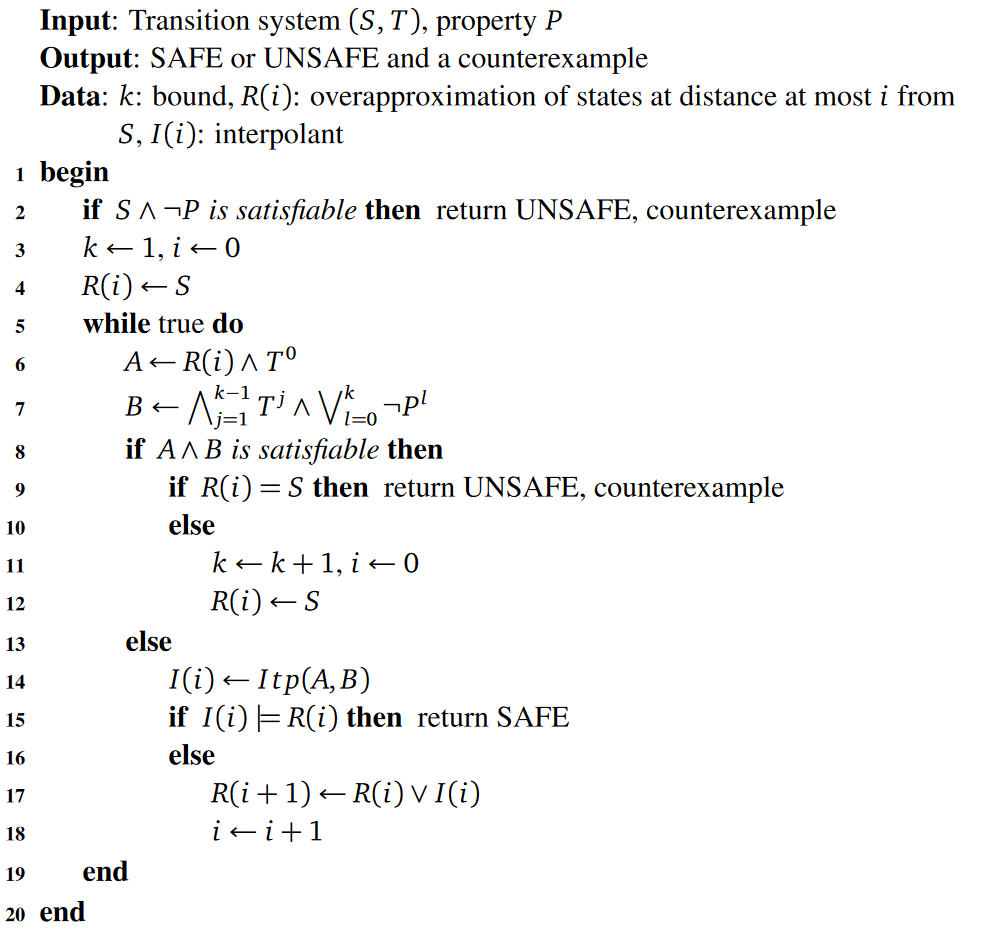
\includegraphics[scale=0.66]{imc-pseudocode.png}
      \caption{Pseudocódigo para IMC retirado de \cite{interpolation2}}
      \label{fig:imcpseudo}
\end{figure}

Considere-se agora a implementação quase direta em Python, através do PySMT:

\usemintedstyle{emacs}

\begin{code}
\begin{minted}{python}
def IMC(TS: TransitionSystem,
        P: FNode,
        S=None,
        customInterpolator=False):

    if not S:
        S = TS.init

    if m := get_model(S & Not(P)):
        print(m)
        return Status.UNSAFE1

    k = 1

    i = 0
    R_i = S.substitute(TS.get_subs(i))

    while True:
        A = R_i & TS.get_unrolling(1)
        B = And(And(TS.get_unrolling(1, k)), Or(get_unrolling(Not(P), k)))
        if m := is_sat(A & B):
            if is_valid(R_i.EqualsOrIff(S)):
                print(m)
                return Status.UNSAFE2
            else:
                k += 1
                i = 0
                R_i = S.substitute(TS.get_subs(i))
        else:
            if customInterpolator:
                I_i = bin_itp(A, B)
            else:
                I_i = binary_interpolant(A, B)

            if is_valid(I_i.Implies(R_i)):
                print(f"Proved at step {i + 1}")
                return Status.SAFE
            else:
                R_i = R_i | I_i
                i += 1
\end{minted}
\caption{Implementação em PySMT do algoritmo de IMC retirado de \cite{interpolation2}}
\label{code:imc}
\end{code}

A versão com comentário encontra-se no anexo em~\ref{code:imc_commented}, ou no GitHub com
o resto do código fonte, também no anexo~\ref{apndx:github}.

\section*{Interpolante de Craig, escolha de lógica SMT}

Para implementar este algoritmo, foi necessário utilizar o teorema de interpolação de
Craig\footnote{\url{https://en.wikipedia.org/wiki/Craig_interpolation}}, que já estava
\href{https://en.wikipedia.org/wiki/Craig_interpolation}{implementado no PySMT}.

É preciso notar que a implementação do PySMT não suporta todas as lógicas \smtlib.
Por exemplo, no caso do estudo em ~\ref{chap:case_study}, a lógica $\text{QF_BV}$\footnote{\url{https://smtlib.cs.uiowa.edu/logics-all.shtml#QF_BV}}
é suficiente para considerar o problema.

No entanto, se não for \textbf{explicitamente} selecionada, o PySMT escolherá
a lógica mais geral que conseguir, que no caso era $\text{QF_AUFBVLIRA}$\footnote{\url{https://smtlib.cs.uiowa.edu/logics-all.shtml#QF_AUFLIA}}, que
não tem, à data da submissão do projeto, uma implementação de um algoritmo para
cálculo do interpolante de Craig entre duas fórmulas arbitrárias.

\section{Interpolante utilizando noção de WPC e SPC}

\newpage
\section{\pdr}

\chapter{Caso de Estudo}\label{chap:case_study}

Para testar a ferramenta desenvolvida, escolheu-se um exemplo simples mas não trivial
de um \fots visto num dos trabalhos práticos da UC de \href{https://paper.dropbox.com/doc/LC-2021-2022-Trabalhos-Praticos-NZEwyS6N5YQQTw1XsYimE#:uid=036036509450795602269559&h2=Trabalho-4}{\lc}.

Considere-se o seguinte problema:

\begin{figure}[H]
      \centering
      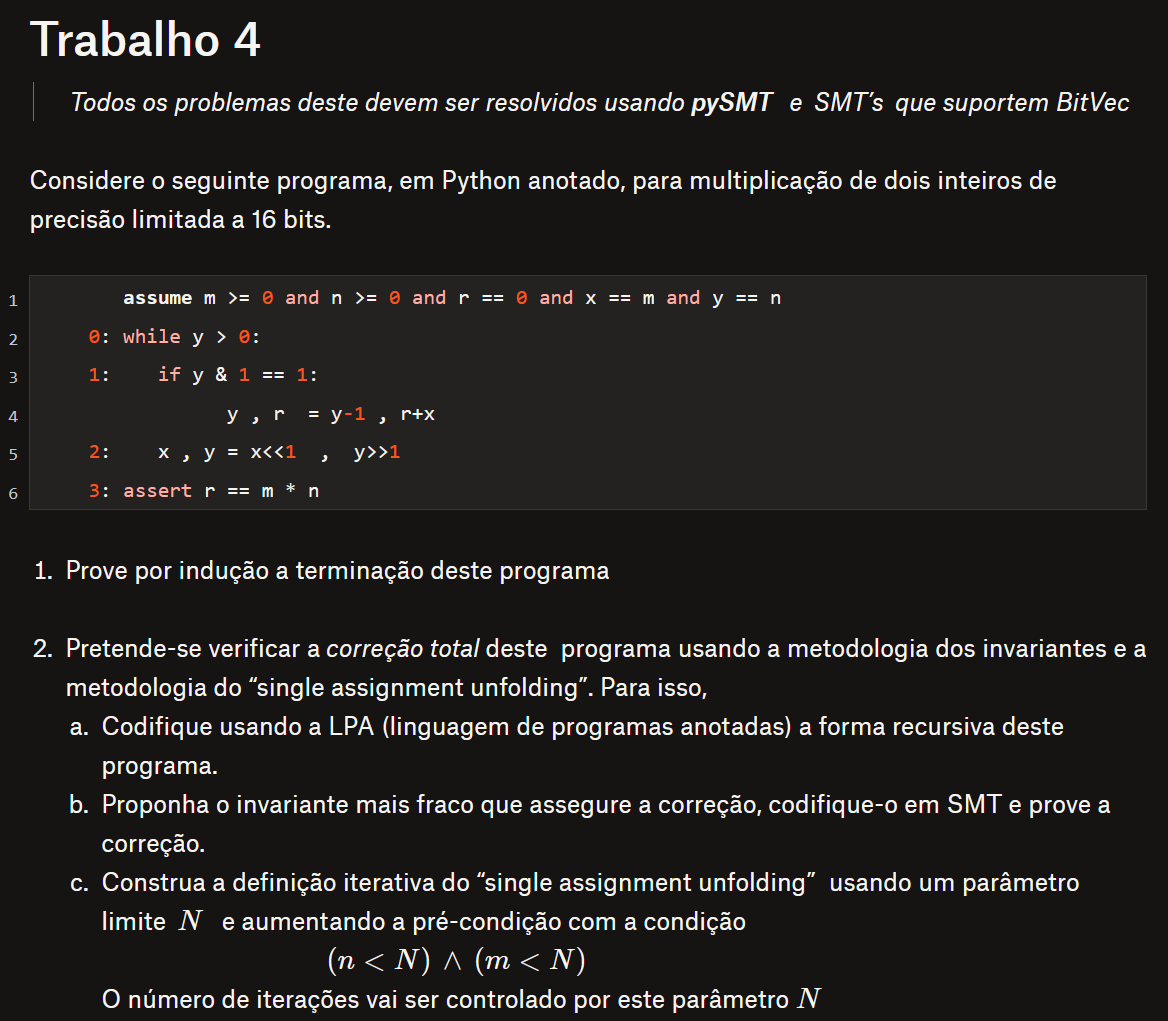
\includegraphics[scale=0.75]{lc-trab4.png}
      \caption{FOTS de trabalho 4 de \lc, ano letivo 2021/2022}
      \label{fig:trab4}
\end{figure}

Abaixo está uma possível codificação do problema acima.

\begin{code}
\begin{minted}{python}
def trab4FinalSimplification(bit_count):
    from pysmt.typing import BVType

    # Variables
    x = Symbol("x", BVType(bit_count))
    m = Symbol("m", BVType(bit_count))
    n = Symbol("n", BVType(bit_count))
    y = Symbol("y", BVType(bit_count))
    r = Symbol("r", BVType(bit_count))
    pc = Symbol("pc", BVType(bit_count))

    npc = next_var(pc)
    ny = next_var(y)
    nx = next_var(x)
    nr = next_var(r)

    from util.transition import TransitionPredicate

    T = TransitionPredicate()

    # pc = 0 ∧ y > 0 -> pc′ = 1                  enters WHILE
    T.add(pc.Equals(0) & (y > 0), npc.Equals(1))
    # pc = 0 ∧ y ≤ 0 -> pc′ = 3                 doesn't enters WHILE
    T.add(pc.Equals(0) & (y <= 0), npc.Equals(3))
    # pc = 1 ∧ y & 1 = 1 -> y′ = y − 1 ∧ r′ = r + x ∧ pc′ = 2      IF condition is true
    T.add(pc.Equals(1) & (y & 1).Equals(1), npc.Equals(2) & ny.Equals(y - 1) & nr.Equals(r + x))
    # pc = 1 ∧ y & 1 ≠ 1 -> pc′ = 2                      IF condition is false
    T.add(pc.Equals(1) & (y & 1).NotEquals(1), npc.Equals(2))
    # pc = 2 -> y′ = y >> 1 ∧ x′ = x << 1 ∧ pc′ = 0      loop back after attributions
    T.add(pc.Equals(2), npc.Equals(0) & nx.Equals(x << 1) & ny.Equals(y >> 1))
    # pc = 3         end of program
    T.add(pc.Equals(3))

    pre = ((m >= 0) &  # m ≥ 0
           (n >= 0) &  # n ≥ 0
           r.Equals(0) &  # r = 0
           x.Equals(m) &  # x = m
           y.Equals(n)  # y = n
           )

    init = pc.Equals(0) & pre
    return TransitionSystem(init, T.get())
)
\end{minted}
\caption{Representação em PySMT de FOTS em ~\ref{fig:trab4}}
\label{code:trab4_fots}
\end{code}

Note-se que é possível definir um FOTS correspondente a um sistema de várias formas.
Neste caso escolheu-se introduzir a variável $pc$ de forma a usar as técnicas estudadas
para fazer provas que envolvessem terminação e animação.

\chapter{Conclusão} \label{chap:concl}

Conclui-se desta forma a apresentação do trabalho desenvolvido pelos autores
para a UC \proj no ano letivo 2021/2022.

\section{Comentários}

\section{Trabalho Futuro}

\appendix % apendice
\chapter{Excertos de Código Utilizado no Projeto} \label{apndx:samples}

\begin{code}
\begin{minted}{python}
def IMC(TS: TransitionSystem,
        P: FNode,
        S=None,
        customInterpolator=False):

    if not S:
        S = TS.init

    # first makes sure P is not violated by S
    if m := get_model(S & Not(P)):
        # halt return a counterexample
        print(m)
        return Status.UNSAFE1

    # bound
    k = 1

    # overapproximation of states at distance at most i from S
    i = 0
    R_i = S.substitute(TS.get_subs(i))

    # for a bound k and a current overapproximation R(i) of the states at distance at
    # most i from S, the algorithm checks if P is violated by the states reachable
    # from R(i) in at most k steps.
    while True:
        A = R_i & TS.get_unrolling(1)
        B = And(And(TS.get_unrolling(1, k)), Or(get_unrolling(Not(P), k)))
        if m := is_sat(A & B):
            # the error might be real or spurious, caused by an insufficient value of k
            if is_valid(R_i.EqualsOrIff(S)):
                # error is real so the system is unsafe
                print(m)
                return Status.UNSAFE2
            else:
                # error is spurious so k is increased to allow finer
                # overapproximations, and the algorithm restarts from S.
                k += 1
                i = 0
                R_i = S.substitute(TS.get_subs(i))
        # R(i) ⋀_{j=0}^{k−1} T^j ⋁_{l=0}^k ¬P^l is unsat
        else:
            # an interpolant I(i) is computed, which represents an approximation of the
            # image of R(i) (i.e., of the states reachable from R(i) in one step).
            if customInterpolator:
                I_i = bin_itp(A, B)
            else:
                I_i = binary_interpolant(A, B)

            # a fixpoint check is carried out: if I(i) |= R(i), it means that all
            # states have been covered, and the system is safe; otherwise, R(i + 1) is
            # set to R(i) ∨ I(i) and the procedure continues.
            if is_valid(I_i.Implies(R_i)):
                # the current R(i) corresponds to an inductive invariant P̂ stronger
                # than P: on one side, S |= R(i), moreover R(i) ∧ T |= I'(i) and I(i)
                # |= R(i) imply R(i) ∧ T |= R'(i); on the other side, the fact that at
                # each iteration 0 ≤ h ≤ i, R(h) ∧ ⋀_{j=0}^{k−1} T |= ⋀_{l=0}^k P^l,
                # together with R(i) being an inductive invariant, yield R(i) |= P.
                print(f"Proved at step {i + 1}")
                return Status.SAFE
            else:
                R_i = R_i | I_i
                i += 1
\end{minted}
\caption{Implementação comentada do algoritmo de IMC -\cite{interpolation2}}
\label{code:imc_commented}
\end{code}

\chapter{Repositório \textit{GitHub} com código fonte e documentação} \label{apndx:github}

\section*{``\textit{Source code}''}

O código fonte da ferramenta desenvolvida é accessível através do link: \url{https://github.com/Alef-Keuffer/FOTS-Prover}.

Está sediado numa página de GitHub de um dos autores.

\section*{Documentação da ferramenta}

A documentação da ferramente encontra-se disponível \href{https://alef-keuffer.github.io/FOTS-Prover.docs/backend.html}{aqui}.

\newpage

%-- Fim do documento -- inserção das referencias bibliográficas

%\bibliographystyle{plain} % [1] Numérico pela ordem de citação ou ordem alfabetica
\bibliographystyle{alpha} % [Hen18] abreviação do apelido e data da publicação
%\bibliographystyle{apalike} % (Araujo, 2018) apelido e data da publicação
                             % --para usar este estilo descomente no inicio o comando \usepackage{apalike}

\bibliography{citations} %input do ficheiro de referencias bibliograficas

\end{document}